\subchapter{Setting up Ethernet communication}{Objectives: Set up 
a local network connection between your computer and the \devboard.}

\section{Connect the host to the \devboard Board}

With a network cable, connect the Ethernet port of your board to the
one of your computer. If your computer already has a wired connection
to the network, your instructor will provide you with a USB Ethernet
adapter. A new network interface, probably \code{eth1} or \code{eth2},
should appear on your Linux system.

To configure this network interface on the workstation side, click on
the {\em Network Manager} tasklet on your desktop, and select {\em
  Edit Connections}.

\begin{center}
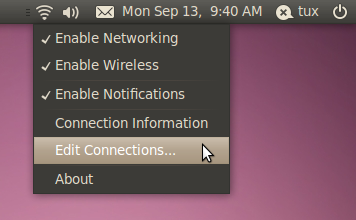
\includegraphics[width=8cm]{labs/setup-network/network-config-1.png}
\end{center}

Select the new {\em wired network connection}:

\begin{center}
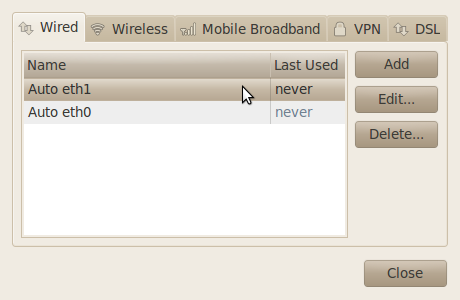
\includegraphics[width=8cm]{labs/setup-network/network-config-2.png}
\end{center}

In the \code{IPv4 Settings} tab, press the \code{Add} button
and make the interface use the SERVER\_IP static IP address,
you selected when you edited \code{host.mk} (default \serverip) (of course, make sure that this
address belongs to a separate network segment from the one of the main
company network).

\begin{center}
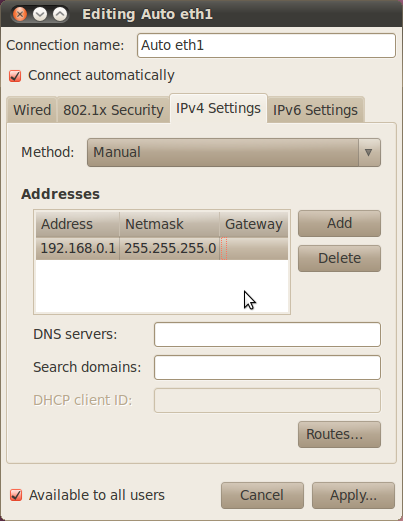
\includegraphics[width=8cm]{labs/setup-network/network-config-3.png}
\end{center}

You can use \code{255.255.255.0} as \code{Netmask}, and leave the
\code{Gateway} field untouched (if you click on the \code{Gateway} box, you
will have to type a valid IP address, otherwise you won't be apply to
click on the \code{Apply} button).

In \code{Ubuntu 14.04}, you can supply \code{24} as \code{Netmask}.

The board must also be configured, but this will be done later in the U-Boot lab.

The network port will be present, but its IP address will only be allocated when
you have a physical connection from the port to the \devboard.

When you have a running \devboard with a cable inbetween later, you can check by:

\begin{verbatim}
ifconfig
\end{verbatim}

